% !TEX encoding = windows-1250
\documentclass[12pt, oneside, a4paper]{mwbk}
\usepackage[cp1250]{inputenc}
\usepackage[polish]{babel}
\usepackage[OT4]{fontenc}

\usepackage{listings}
\lstset
{
	captionpos=b,
	basicstyle=\footnotesize\ttfamily,
	frame = single,
	tabsize = 3,
	breaklines = true
}
\renewcommand\lstlistlistingname{Spis listing�w}

\usepackage{graphicx}
\usepackage{verbatim}

\usepackage{enumitem}
\usepackage[noend]{algorithmic}
\usepackage[ruled]{algorithm}

\usepackage{color}
\usepackage[normalem]{ulem}

\usepackage{rotating}
\usepackage{float}
\usepackage{textpos}

\linespread{1,3}
\oddsidemargin = 10pt
\textwidth = 470pt

\hyphenpenalty=1000
\tolerance=500

\begin{document}
\author{Krzysztof Szczech}
\title{Tytu�}
\begin{titlepage}
\thispagestyle{empty}
\begin{textblock}{1}(-2.65,-1.65)

\includegraphics{figures/tytulowa_pusta_mgrinz.pdf}
\end{textblock}
\vspace{7.3cm}
\begin{center}
\fontfamily{ptm}
\selectfont
\Huge
Wybrane aspekty techniczne odwzorowania artystycznej wizji jako tr�jwymiarowego �rodowiska w grze komputerowej
\end{center}
\begin{center}
\fontfamily{ptm}
\selectfont
Praca dyplomowa in�ynierska
\end{center}
\vspace{5.6cm}
\begin{center}
\fontfamily{ptm}
\selectfont
\hspace{-1cm}
\begin{tabular}{l}
Wydzia� Fizyki Technicznej, Informatyki i Matematyki Stosowanej \\
Promotor: dr in�. Rafa� Szrajber \\
Dyplomant: Krzysztof Szczech \\
Nr albumu: 180707 \\
Kierunek: Informatyka \\
Specjalno��: Technologie gier i symulacji komputerowych
\end{tabular}
\end{center}
\vspace{-.5cm}
\begin{center}
\fontfamily{ptm}
\selectfont
\begin{textblock}{13}(0,0.2)
��d�, 2016
\end{textblock}
\end{center}
\end{titlepage}



\tableofcontents

% !TeX encoding = windows-1250
\chapter{Wst�p}
\label{t:int}
Bardzo szybki - trwaj�cy od kilku dziesi�cioleci - rozw�j komputer�w pozwoli� na przenoszenie coraz bardziej z�o�onych fragment�w otaczaj�cego nas �wiata na ekrany monitor�w. Jeste�my w stanie symulowa� skomplikowane zjawiska przyrody, co pozwala nam lepiej zrozumie� �wiat na kt�rym �yjemy, "budowa�"  wirtualne domy w kt�rych kiedy� b�dziemy chcieli zamieszka� w rzeczywisto�ci, czy te� tworzy� pi�kne obrazy bez pomocy p��tna i p�dzla.\newline

\section{Cel i za�o�enia pracy}

\section{Zakres pracy}


\newpage
\thispagestyle{empty}
\begin{textblock}{1}(-2.65,-1.65)
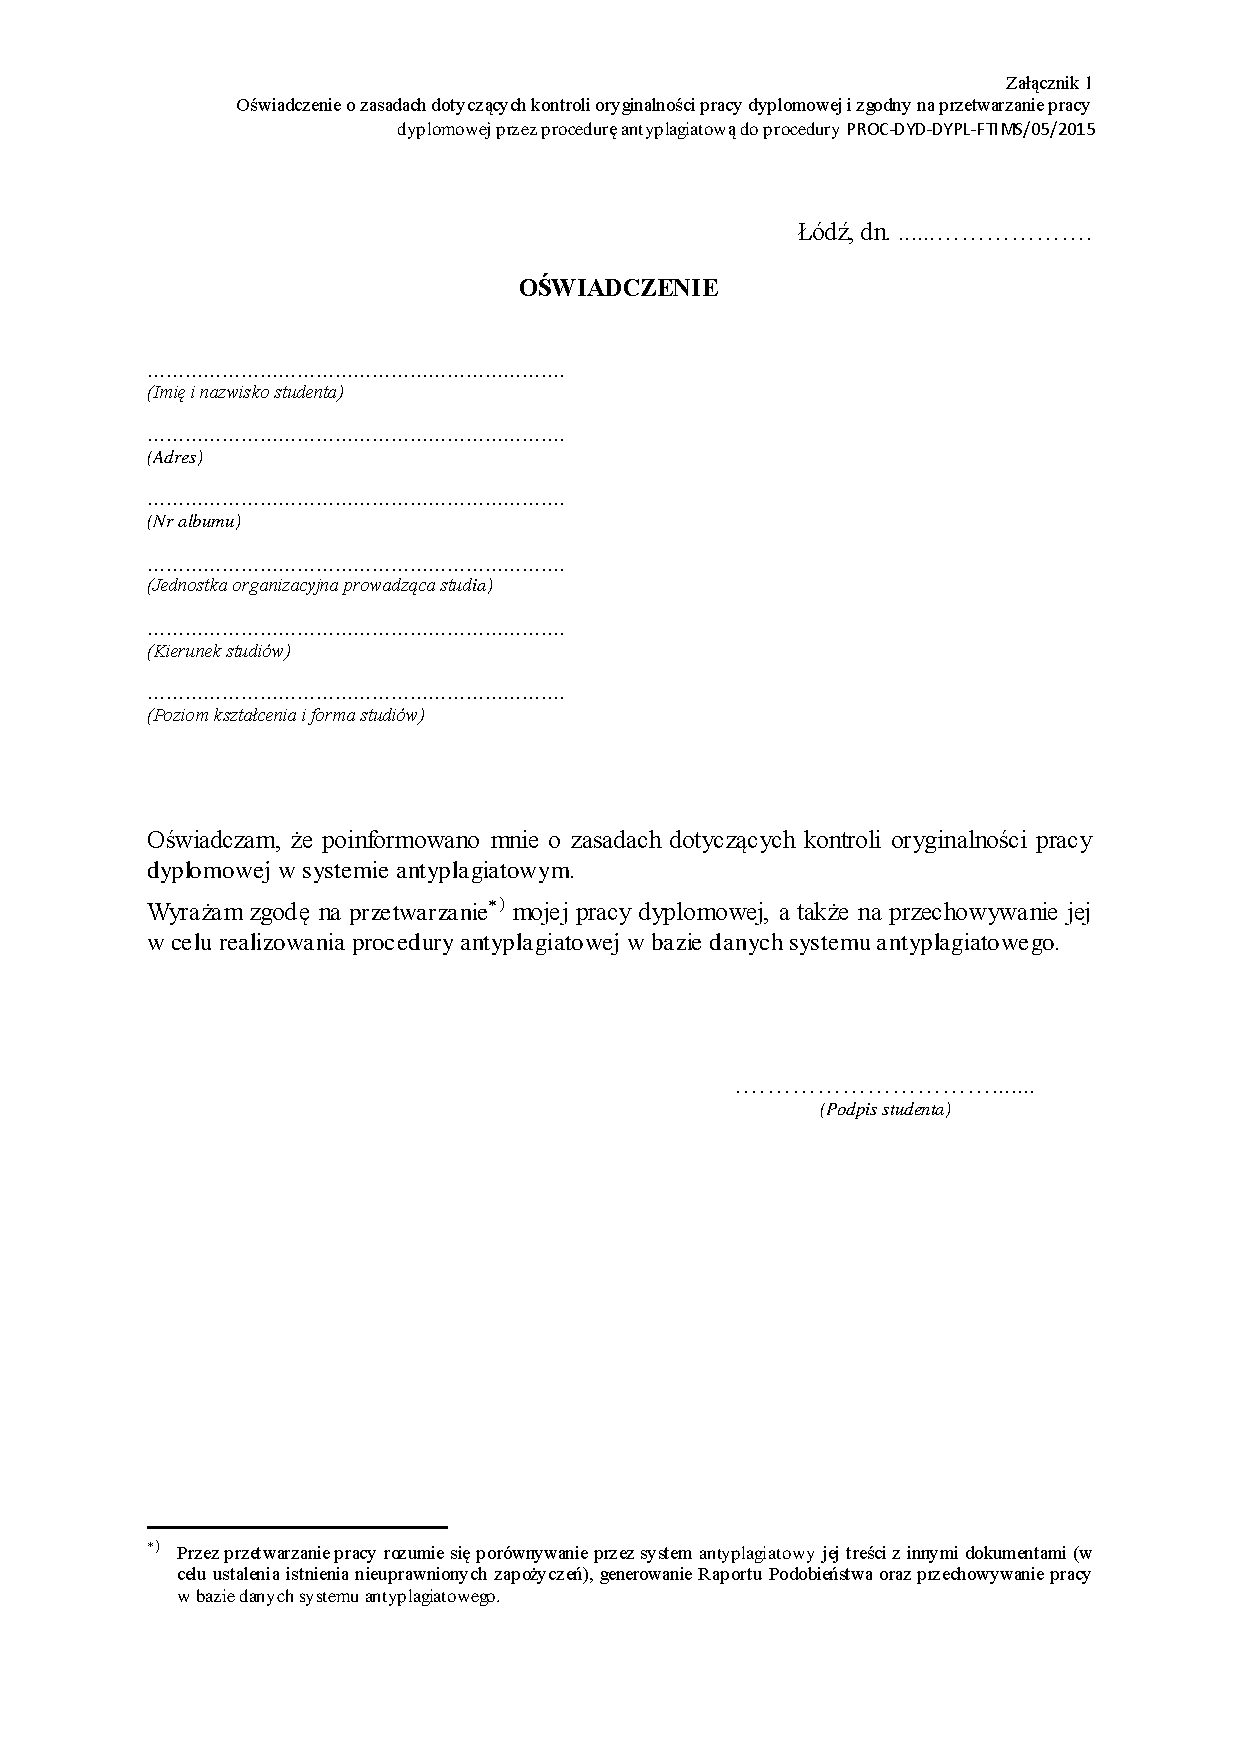
\includegraphics{figures/Zal_1.pdf}
\end{textblock}

\newpage
\thispagestyle{empty}
\begin{textblock}{1}(-2.65,-1.65)
	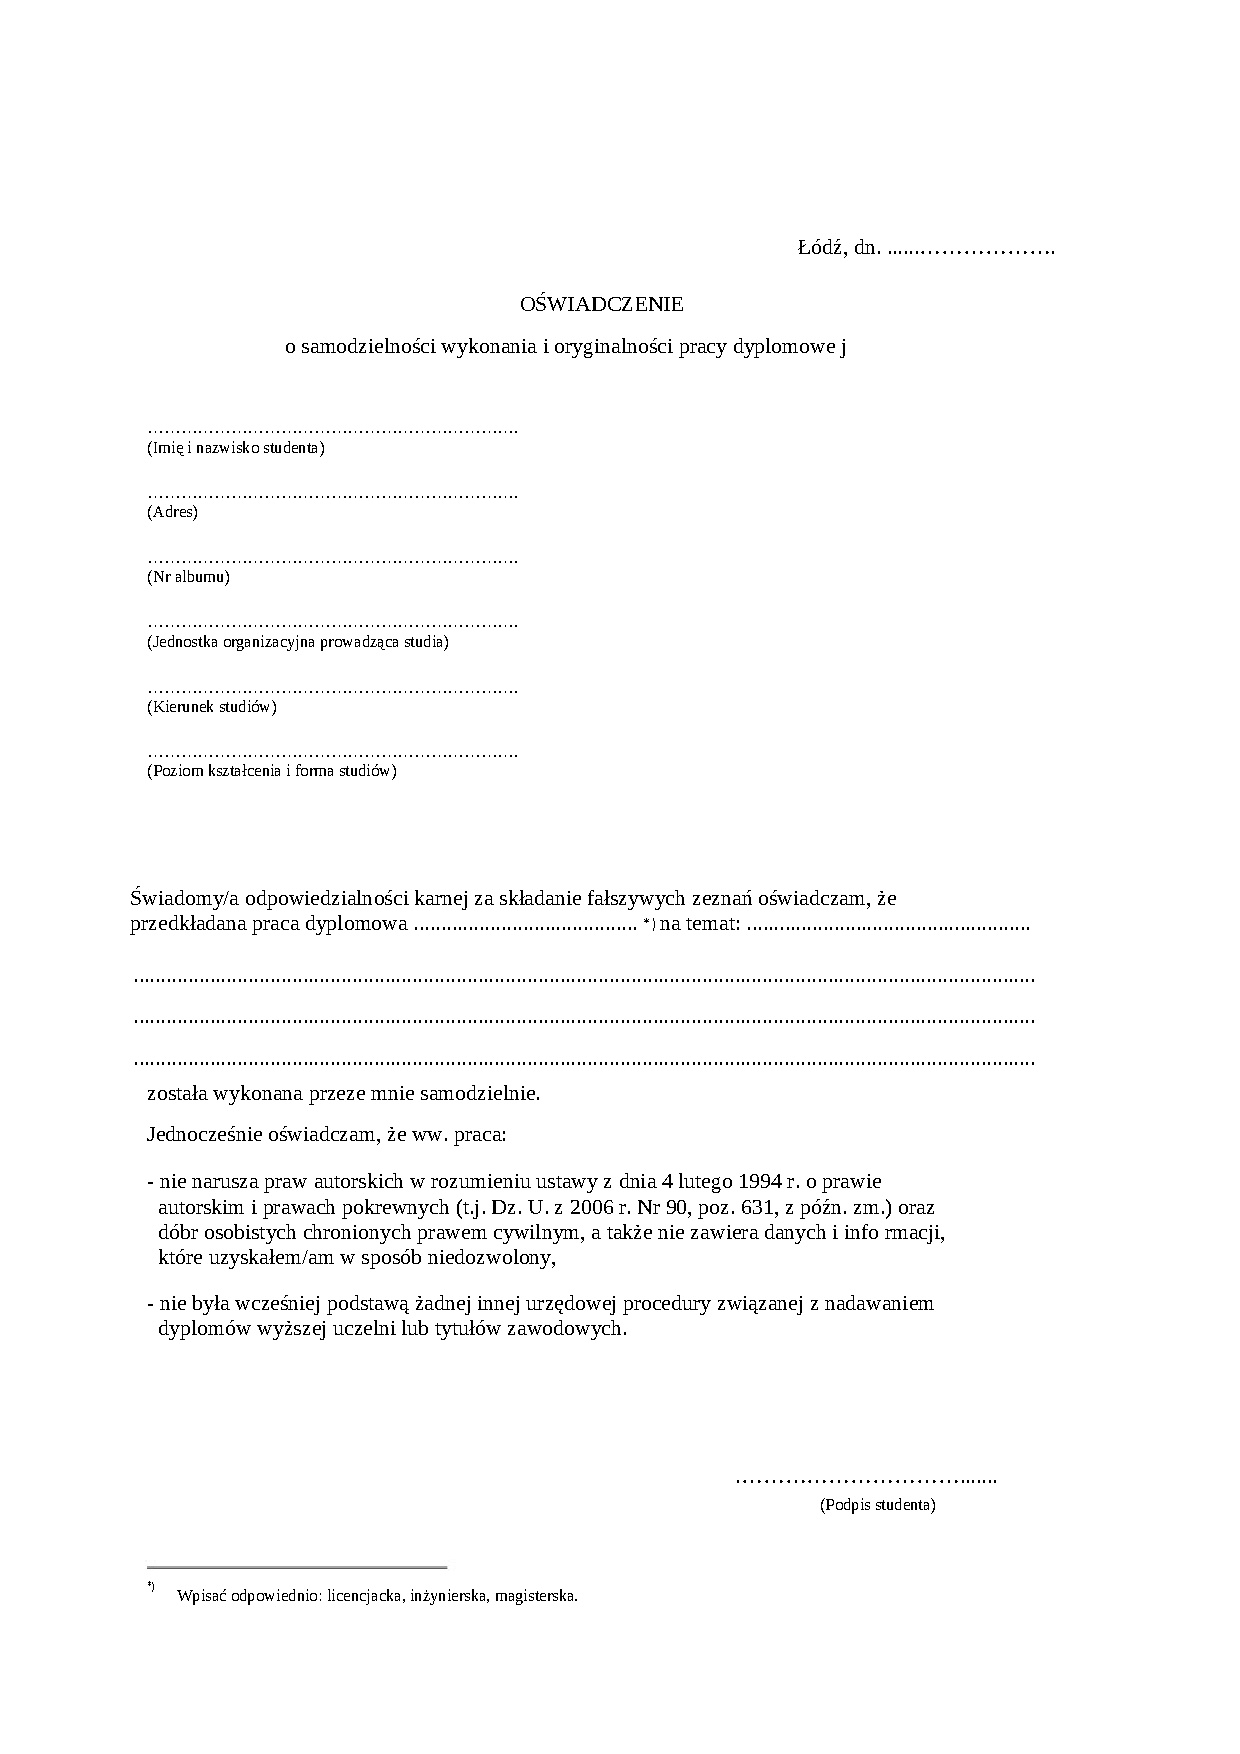
\includegraphics{figures/Zal_2.pdf}
\end{textblock}

\newpage
\thispagestyle{empty}
\begin{textblock}{1}(-2.65,-1.65)
	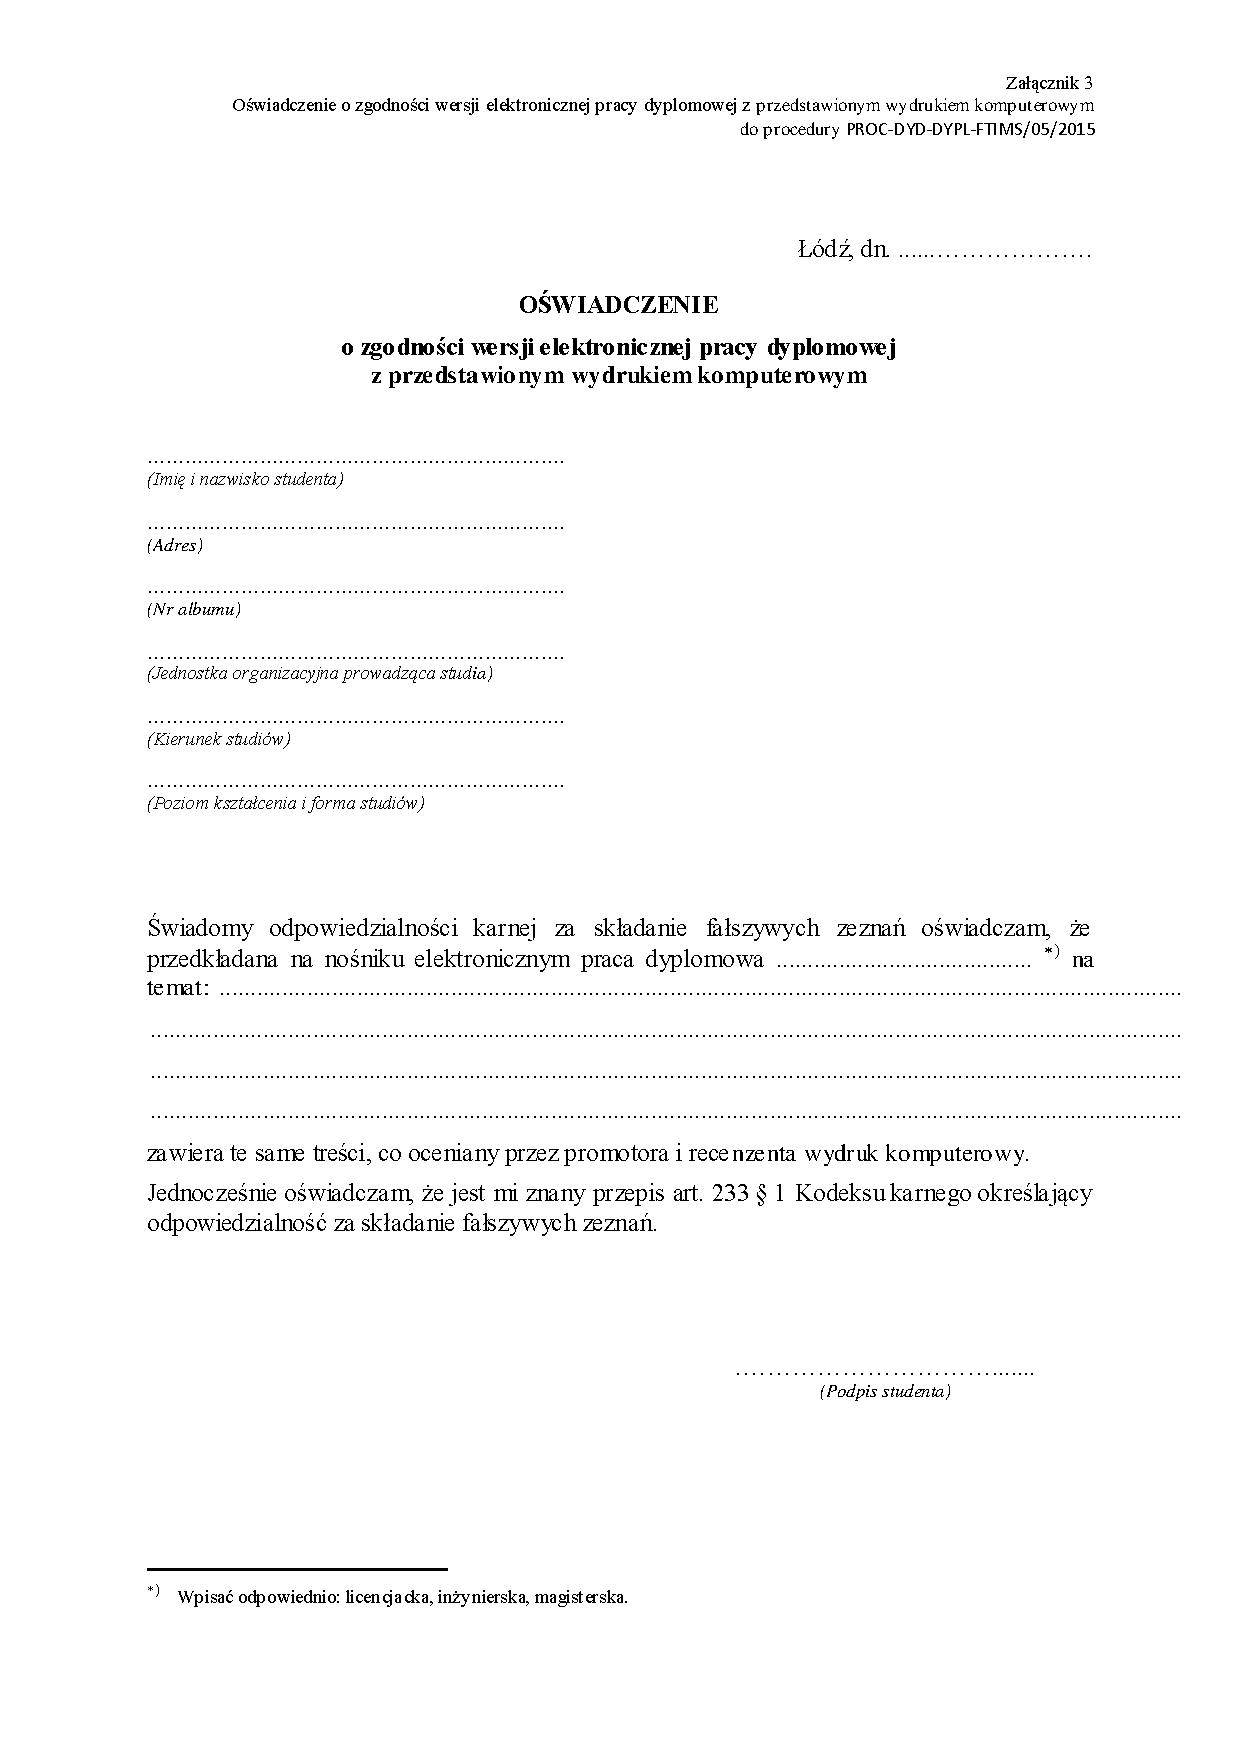
\includegraphics{figures/Zal_3.pdf}
\end{textblock}

\end{document}
